\chapter{Air Quality}\label{ch:air_quality}
\chapterauthor{TBD\footnote{Statement of Contributions: }}

\section{Air Masks in Asia}

\subsection{Air Pollution and Air-Borne Contagions}

A common site in East Asia, people wearing masks. Even designer mask coming in vogue suggests that the ...


Kintisch, Eli. "Department of State's air pollution sensors go global." (2018): 248-249.


On April 4th, 2018 off the coast of the island of Borneo an oil spill engulfing much of the East Asian sea sweep Indonesia making it go on a state of emergency. Southeast Asia's abundance of temperate rainforest make it even more important to mitigate hazardous air pollution in the region. Air pollution is seen in Indonesia with the sizeable burning of land systems contributing to record high air hazards each year. The movement of CO2 in Southeast Asia activity show shifts in the regions 

Research on CO and CO2 concentration have shown high activity increase in the southern and northern Indian ocean. The increase was from approximately 50 ppbv in southern hemisphere to >120 ppbv north of the equator. CO findings also report as high as 200 ppbv near coastal India. We can also see relative aersoal mass in ozone levels indicating common transport and source for CO as well. \citep{phadnis2002evolution}

\subsection{Southeast Asia Haze}

\begin{figure}[ht]
  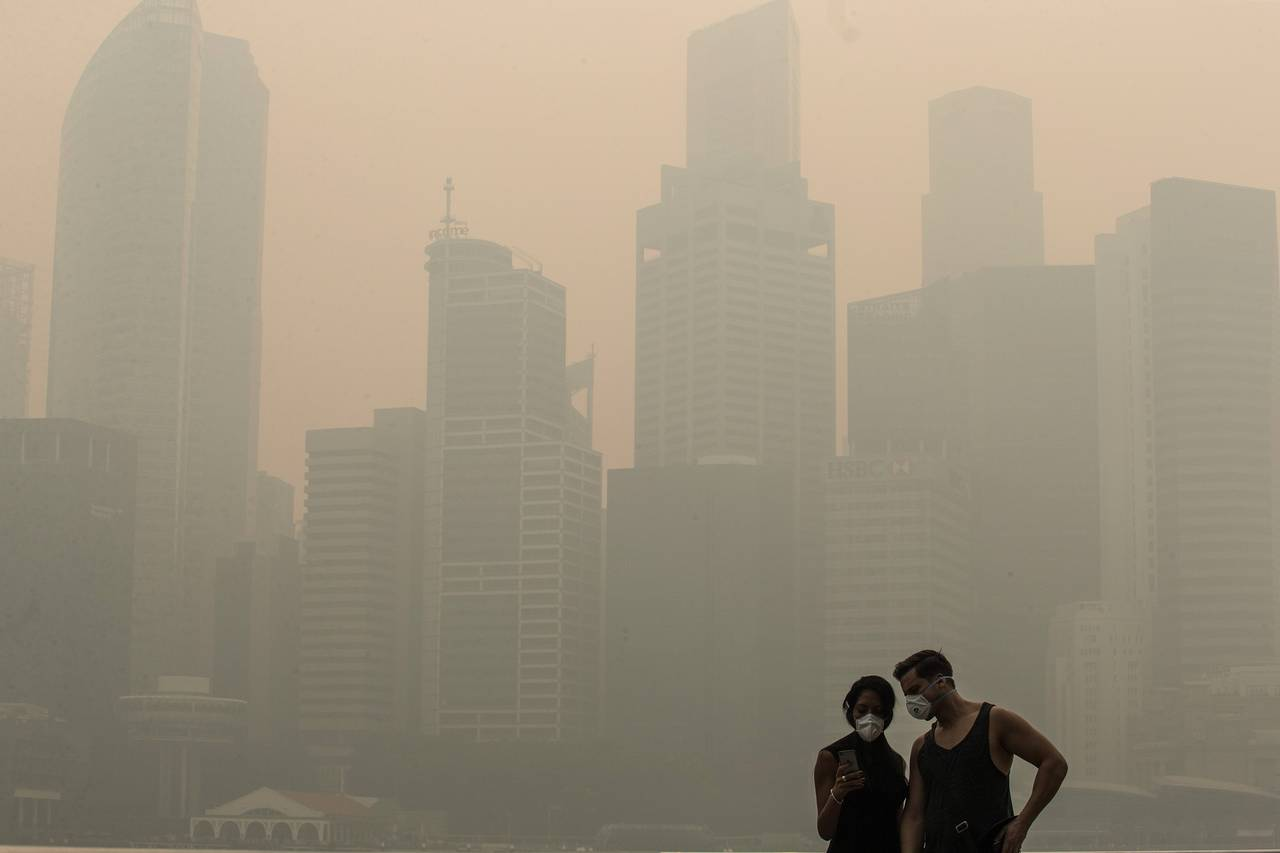
\includegraphics[width=\linewidth]{SoutheastAsianHaze.jpg}
  \caption{Southeast Asian Haze in Indonesia}
  \label{fig:southeastasiahaze}
\end{figure}

The Southeast Asia Haze has become infamous for its impacts on human health and agriculture. In many parts of Southeast Asia, the haze has become an annual phenomenon as human activity in the region, including prescribed peatland burns, becomes more prevalent (figure \ref{fig:southeastasiahaze}). The Indian Ocean Experiment (INDOEX) study done in 1999 found that the aerosols in the haze could drastically disrupt water availability and crop production because of the way the aersols interfere with the sunlight's breakdown of hydroxl radicals \citep{taylor2003abcs}. There is a tremendous loss of biodiversity because the haze can cover millions of hectacres of land for prolonged periods of time. The haze pollution has both immediate and long-term environmental impacts. Though an overwhelming number of the massive forest fires occur in Indonesia, the haze crosses national boundaries and is carried by winds to several neighboring countries, such as Malaysia and Singapore.    

The burning of peat, as compared to the burning of other kinds of land, is much more dangerous because of the particular matter and sulphur and nitrous oxides that are released when peat is burned. The Southeast Asian Haze is unique because of the impact that burning peat has on the atmosphere. 

The impact that the Southeast Asia Haze has had on human health is drastic and worsened in recent years. There are long-term respiratory effects of the haze. Air pollution indexes from the World Health Organization reached extremely unsafe levels because the biomass smoke contained soot particles, inorganic materials like silica, ammonia, and more \citep{sastry2002forest}. This air pollution can cause respiratory and cardiovascular diseases, of which the elderly and young are most vulnerable. Premature deaths from the haze are difficult to measure because it is on a much longer time-scale than immediate respiratory problems, but it is suggested that the haze in Southeast Asia will have long-term impacts on human health.

There are not only environmental and health impacts but also economic and political impacts from the Southeast Asia haze. The negative impacts the haze has on human health and agriculture cost Southeast Asian nations billions of USD in damage and should the magnitude of the Southeast Asian haze continue, future profits and ecological health could be permanently damaged. Future profits and ecological health are at risk, even if the phenomenon of the Southeast Asia haze is resolved, because the landscape could be damaged and take centuries to recover properly.

\begin{figure}
  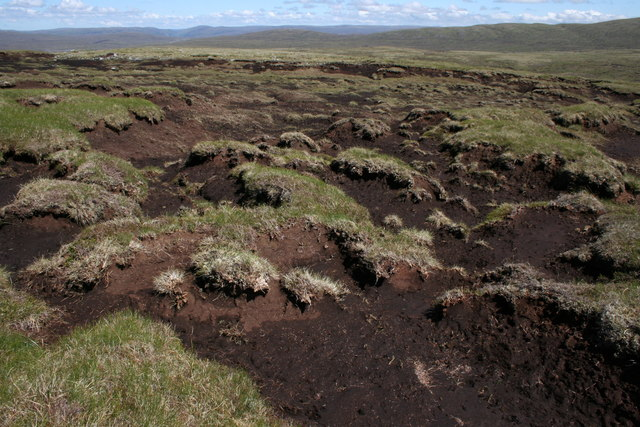
\includegraphics[width=\linewidth]{peaterosion.jpg}
  \caption{Peat Erosion}
  \label{fig:peaterosion}
\end{figure}

\subsubsection{ENSO Events}

The El Ni\~{n}o-Southern Oscillation (ENSO) phenomenon is a cyclical warming of the eastern equatorial Pacific Ocean. It occurs every three to five years and lasts anywhere from six to eighteen months (figure \ref{fig:elnino}). ENSO, unlike La Nina, brings droughts to even the wettest parts of insular Southeast Asia, such as Borneo \citep{aiken2004runaway}.

Peatlands are particularly vulnerable to ENSO because it is so dependent on consistent moisture for freely draining soil. Droughts cause water levels in peat swamps to drop. In Borneo, peat swamp forests during severe El Nino droughts have been subject to fires that have consumed peat up to 50cm in the late twentieth century \citep{turetsky2015global}.

In El Nino drought years, the prescribed burns in peatlands can burn with greater intensity than in more climatically stable years. With dry lakes, low river levels, and dry peat soils, strong winds during El Nino can help ignite fires or spread fires that had already been started intentionally by human activity \citep{chokkalingam2005fire}.  

\begin{figure}
  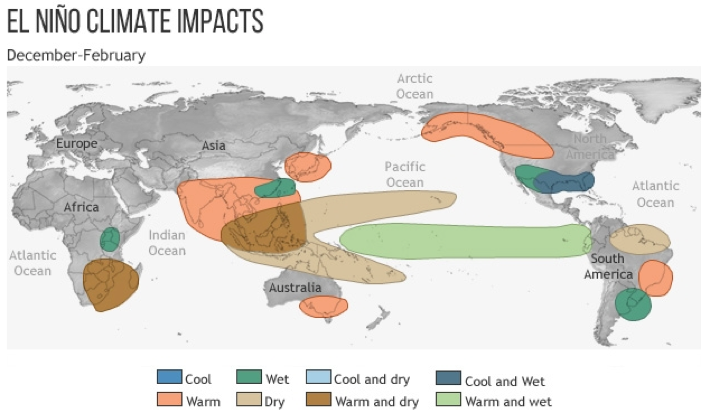
\includegraphics[width=\linewidth]{elnino.png}
  \caption{A model of global El Nino climate impacts during the peak of an El Nino-Southern Oscillation event.}
  \label{fig:elnino}
\end{figure}

The ENSO phenomenon that led to drought conditions was associated with high air pressure over the region that prevented the smoke haze from dissipating. As a result, the haze spread horizontally but managed to maintain a high level of concentration. In cities, the haze led to an atmospheric inversion and trapped emissions from cars and factories within the city. The high air pressure makes it difficult for the smoke haze to dissipate in cities in Southeast Asia because there is a large mass of high-rise buildings in the cities. The exact causes of the trapped haze are still unknown but one theory is that it is similar to the heat island effect, in which changes to the landscape cause urban regions to become warmer than their rural surroundings. 